%----------------------------------------------------------------------------
\chapter*{Bevezető}\addcontentsline{toc}{chapter}{Bevezető}
%----------------------------------------------------------------------------

% Gyakorlás szerepe a tanulásban
A tanulás egy nehéz és időigényes folyamat, melynek megértésével és tökéletesítésével napjainkban is aktívan foglakozik a tudomány.
Ennek a folyamatnak elengedhetetlen része az önállóan végzett feladatmegoldás, a gyakorlás, mely során az elméleti tudás a gyakorlatban is hasznosítható tapasztalattá válik.
Gyakorlás közben fontos, hogy minél gyakrabban -- ha lehet, folyamatosan -- ellenőrizzük munkánk eredményét, ezzel biztosítva azt, hogy ne keletkezzenek rossz berögződések, melyek utólagos kijavítása további időt igényelne.

Az ellenőrzésnek sokféle módja is ismert, mely módozatokat többféle nézőpontból is értékelhetünk.
Az egyik ilyen nézőpont az ellenőrzési módszer flexibilitása, amely azt mutatja meg, mennyire változtatható meg a feladat úgy, hogy az ellenőrzési módszer továbbra is alkalmazható maradjon.
A spektrum egyik végén állnak az inflexibilis módszerek, amilyen például egy adott feladathoz mellékelt megoldókulcs.
A legegyszerűbb megoldókulcsok egyedül a feladat elvárt eredményét adják meg, ezért ezek flexibilitása igen csekély, hiszen a feladatban bármilyen érdemi változtatást elvégezve elvesztik érvényességüket. 
Ugyanakkor ezek a leggyorsabb és legolcsóbb módszerek, hiszen egyetlen összehasonlítás szükséges a saját és a megoldókulcs által megadott érték között, a megoldókulcsok pedig minimális költséggel sokszorosíthatóak és felhasználhatóak.
A spektrum másik végén találhatóak a flexibilis módszerek, amilyen például az oktatók -- általános esetben az adott terület szakértőinek -- alkalmazása, akik a feladat témakörében való jártasságuk révén gyakorlatilag bármely megoldás ellenőrzésére képesek.
Az oktató azonban drága erőforrás, mind időben, mind pénzben, hiszen egy adott téma szakértőjeként a tanulók feladatainak ellenőrzése helyett az iparban is nagy szükség lenne rá.
Ebből fakadóan -- sok oktató alkalmazása költséges, ugyanakkor az iparnak nagyszámú szakértőre van szüksége -- az egy oktatóra eső hallgatók száma igen magas, amely körülmény nem kedvez az oktatás színvonalának, hiszen így minden hallgatóra kevesebb ideje jut az oktatónak.
E két véglet között megannyi módszert találunk, amelyek alkalmazhatósága nagyban függ a feladat jellegétől és témakörétől.

Az oktatók alkalmazásának van azonban egy másik nagy előnye is: a tanulók eredményessége egy független személy által is értékelésre kerül.
Enélkül az oktatási és egyéb akkreditációs intézmények legitimitása megszűnne, működésük értelmét vesztené.

Napjainkban a költségcsökkentés egyik leggyakoribb formája még mindig az automatizálás.
Az első ipari forradalommal a világ rohamos fejlődésnek indult, melyet a második és a harmadik forradalom után most a negyedik követ \cite{FourthRevolution}.
\begin{figure}[h]
    \centering
    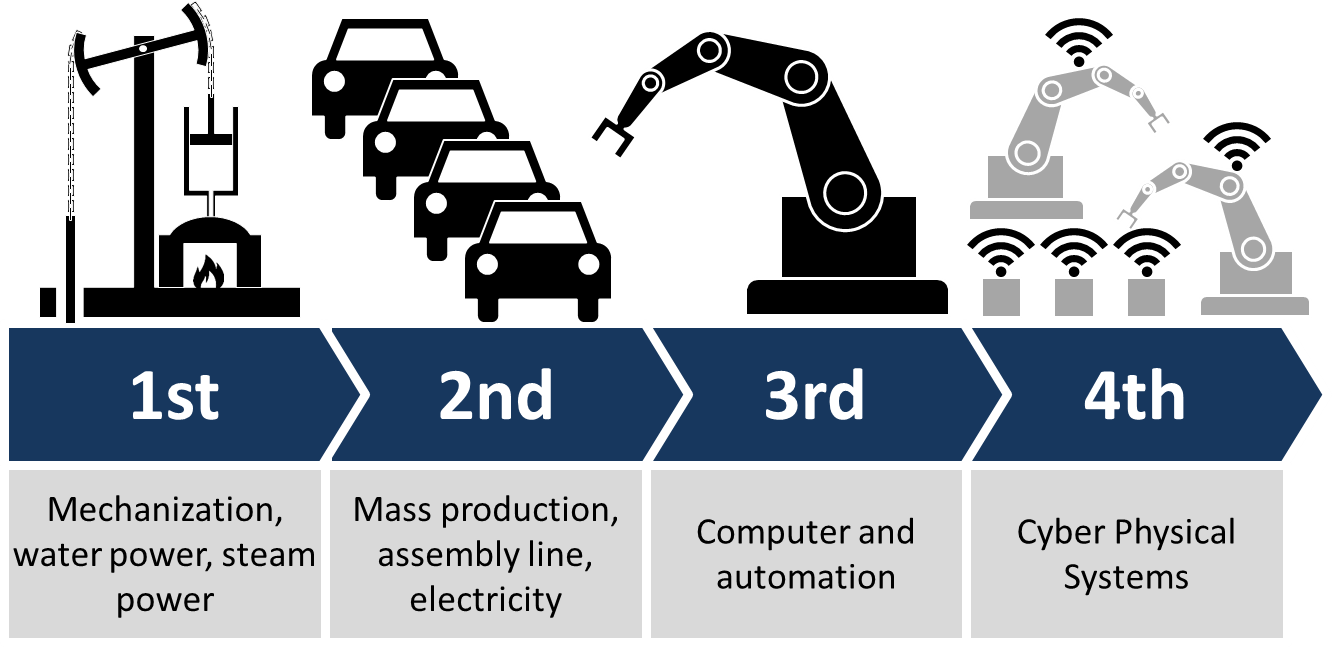
\includegraphics[width=0.8\textwidth]{figures/industrial_revolutions}
    \caption[Ipari forradalmak]{Ipari forradalmak (forrás: Christoph Roser at AllAboutLean.com)} % https://en.wikipedia.org/wiki/Industry_4.0#/media/File:Industry_4.0.png
\end{figure} 
Az automatizálás a harmadik ipari forradalom részeként a számítógépek elterjedésével jelent meg.
A számítógépek lehetővé teszik olyan feladatok automatizálását is, melyek azelőtt lehetetlennek tűntek, ráadásul mindezt egyre olcsóbban.

Ha a számítógépek által nyújtott automatizálás tulajdonságait -- olcsó hardver, könnyen sokszorosítható szoftver, gyors működés, akár igen magas szintű flexibilitás szakértelem (mesterséges intelligencia) hozzáadásával -- vizsgáljuk, könnyű belátni, hogy igen kedvezőek az eddig említett ellenőrzési módszerekkel összevetve.
Ezen gondolatmeneten továbbhaladva eljuthatunk az \textit{automatizált ellenőrzőrendszerek} ötletéhez.
Az automatizált ellenőrzőrendszerek olyan számítógépes szoftverek, melyek a szakértők által előre betáplált logika segítségével képesek bizonyos feladatcsoportok megoldásainak ellenőrzésére.
Ezek a rendszerek különösen jól alkalmazhatóak azokon a területeken, ahol a feladatok helyes megoldásai egyszerű szabályrendszerekkel leírhatóak, ellenőrizhetőek.
Az egyik ilyen terültet a programozás oktatása.

A harmadik ipari forradalom óta, de különösen a negyedik hajnalán, az iparban egyre nagyobb igény mutatkozik informatikai szakemberek iránt, mely az utóbbi években hiányszakmává nőtte ki magát az utánpótlásképzés lassúsága miatt.


\section{Automatizált feladatkiértékelés}
Az automatizált feladatkiértékelés elnevezés elsőre kissé félrevezető lehet, hiszen nem egy adott feladatot kiértékeléséről van szó, hanem a feladatra adott megoldás helyességének ellenőrzéséről.


\section{Online oktatást segítő rendszerek}
% TODO: Feladat indokoltsága: miért/mire jók az online oktatási rendszerek, a feladatbeadó rendszerek, automatikus kiértékelés
%       Eddigi megoldások (Coursera, Khan Academy, edX, Cporta)[http://www.lifehack.org/articles/money/25-killer-sites-for-free-online-education.html], hallgatói és oktatói szemszög


\section{A diplomaterv felépítése}
A dolgozatot az elvégzett munka és továbbfejlesztési lehetőségek összefoglalásával zárom.
